\section{Power and Thermal Models}\label{sec:power_therm_model}

In this section, we present the power and thermal models used in this work. 
% In order to determine the energy-efficient power budget of a multi-core dark silicon system, the 
% we present power modeling and thermal modeling techniques in this section, which are important basic knowledges for our new work.

\subsection{Power model}\label{sec:power_model}

The total power of a chip, denoted as $p$, is composed of dynamic power and static power. The dynamic power, denoted as $p_d$, depends on the activities of the chip, which is expressed as
% \begin{equation}\label{eq:dyn_power}
% p_{d} = \alpha_{d} \cdot V_{dd}^{2} \cdot f,
% \end{equation}
% where $V_{dd}$ stands for the operating voltage, $f$ stands for the clock frequency, and $\alpha_{d}$ is defined as:
% \begin{equation}\label{eq:alpha_d}
% \alpha_{d} = \frac{p_{d_{max}}}{V_{max}^{2}f_{max}},
% \end{equation}
% in which $p_{d_{max}}$ is the dynamic power when the core is at the maximum clock frequency $f_{max}$ and maximum operating voltage $V_{max}$.

% It is assumed the clock frequency $f$ changes with $V_{dd}$ to the lowest allowable point:
% \begin{equation}\label{eq:f_v}
% f = (V_{dd}-V_{th}) \cdot (\frac{f_{max}-f_{min}}{V_{max}-V_{th}})+f_{min}.
% \end{equation}
% where $f_{min}$ stands for the minimum clock frequency, and $V_{th}$ stands for the threshold voltage.

% Yet the static power $p_{s}$ of the chip is caused by leakage current $I_{leak}$ as:
% \begin{equation}\label{eq:sta_power}
% p_{s} = \alpha_{s}\cdot V_{dd} \cdot I_{leak},
% \end{equation}
% where $\alpha_{s}$ is defined as:
% \begin{equation}\label{eq:alpha_s}
% \alpha_{s} = \frac{p_{s_{max}}}{V_{max}\cdot I_{max}},
% \end{equation}
% in which $p_{s_{max}}$ is the static power when the core is running at thermal limit, and $I_{max}$ is the corresponding maximum leakage current. Due to the non-linear relationship between $I_{leak}$ and temperature, static power is also sensitive to temperature, which makes it hard to obtain.

\begin{equation}\label{eq:dyn_power}
p_{d} = C_{eff} \cdot V_{dd}^{2} \cdot f,
\end{equation}
where $V_{dd}$ stands for the operating voltage, $f$ is the clock frequency, and $C_{eff}$ is the effective switching capacitance.

In equation~\eqref{eq:dyn_power}, the clock frequency $f$ and the operating voltage $V_{dd}$ of each modern processor core are changed at runtime (widely known as dynamic voltage and frequency scaling (DVFS)), in order to adjust the core's energy efficiency and performance. 
A widely used model to discribe such relationship between $f$ and $V_{dd}$ is [cite ???]
\begin{equation}\label{eq:f_v}
f = (V_{dd}-V_{th}) \cdot (\frac{f_{max}-f_{min}}{V_{max}-V_{th}})+f_{min}.
\end{equation}
where $f_{min}$ and $f_{max}$ stands for the minimum and maximum clock frequencies, respectively, $V_{th}$ stands for the threshold voltage, and $V_{max}$ stands for ???.

The static power $p_{s}$ of the chip is caused by leakage current $I_{leak}$ as:
\begin{equation}\label{eq:sta_power}
p_{s} =V_{dd} \cdot I_{leak}.
\end{equation}
Due to the nonlinear relationship between $I_{leak}$ and temperature, static power is also sensitive to temperature. $I_{leak}$ is composed mainly by the subthreshold current and gate current~\cite{Liu:DATE'07,ShenTan:TODAES'12,WangWan:TOC'18}, therefore $I_{leak}$ can be approximated as:
\begin{equation}\label{eq:leakage}
I_{leak}=I_{sub}+I_{gate}.
\end{equation}

In~\eqref{eq:leakage}, $I_{gate}$ is considered as a constant because it does not depend on temperature~\cite{WangWan:TOC'18}. Whereas $I_{sub}$ is nonlinearly related to temperature. It can be approximated using a linear model $I_{lin}$ based on Taylor expansion as~\cite{WangWan:TOC'18}:
\begin{equation}\label{eq:sub_current_lin}
  \begin{split}
    I_{sub} \approx & I_{lin} \\
     =& K (\frac{k_b}{q})^2 e^{\frac{q(V_{GS}-V_{th})}{\eta k_b
    T_{p_0}}}\\
&\times ({T_{p_0}}^2 + (2T_{p_0} - \frac{q(V_{GS}-V_{th})}{\eta
  k_b})(T_p-T_{p_0})).
\end{split}
\end{equation}
where $k_b$ is the Boltzmann constant, $q$ is the elementary charge, $T_{p}$ is a scalar representing temperature at one place,~\footnote{$T$
introduced latter in~\eqref{eq:therm_model} is a vector representing temperatures at multiple positions} $K$ and $\eta$ are
process related parameters, $V_{th}$ is the threshold voltage, and $T_{p_0}$ is the Taylor expansion point.

By combing equations \eqref{eq:sta_power}, \eqref{eq:leakage}, and \eqref{eq:sub_current_lin}, we obtain the final static power model in scaler form as:
\begin{equation}\label{eq:sta_power_lin}
\begin{split}
p_s&=V_{dd}I_{leak}\\
&=V_{dd} (I_{lin}+I_{gate})\\
&=V_{dd}(a_p T_p + I_0),
\end{split}
\end{equation}
where $a_pT_p$ is the term formulated by combing all terms (linearly) associated with $T_p$ in \eqref{eq:sub_current_lin},
$I_{0}$ contains constant terms that are not associated with $T_p$ in \eqref{eq:sub_current_lin} and the gate leakage $I_{gate}$.

% \begin{equation}\label{eq:lin_leakage}
% p_{s} =V_{dd} (p_{0}+a_{s} \cdot T).
% \end{equation}
% $p_{0}$ is a constant terms that are not associated with $T$, $a_{s}$ is the coefficient associated with $T$. $P_{0}$ and $A_{s}$ are the constants corresponding for $p_{0}$ and $a_{s}$ in vector/matrix form.


%Apparently, the leakage current has a complex relationship with temperature. In this work, we use \eqref{eq:sta_power}, \eqref{eq:leakage}, and \eqref{eq:sub_current} to model the static power considering such relationship. The parameters of leakage current can be obtained by curve fitting using HSPICE simulation data. In order to see the accuracy of the model used, Fig.~\ref{fig:leakage} shows an HSPICE simulation result of leakage using TSMC \SI{65}{nm} process model and its curve fitting result using approximate leakage model. From the figure, we can see that the static power model has high accuracy for all common temperatures of IC chips.
% \begin{figure}%curve fitting
%   \centering
%   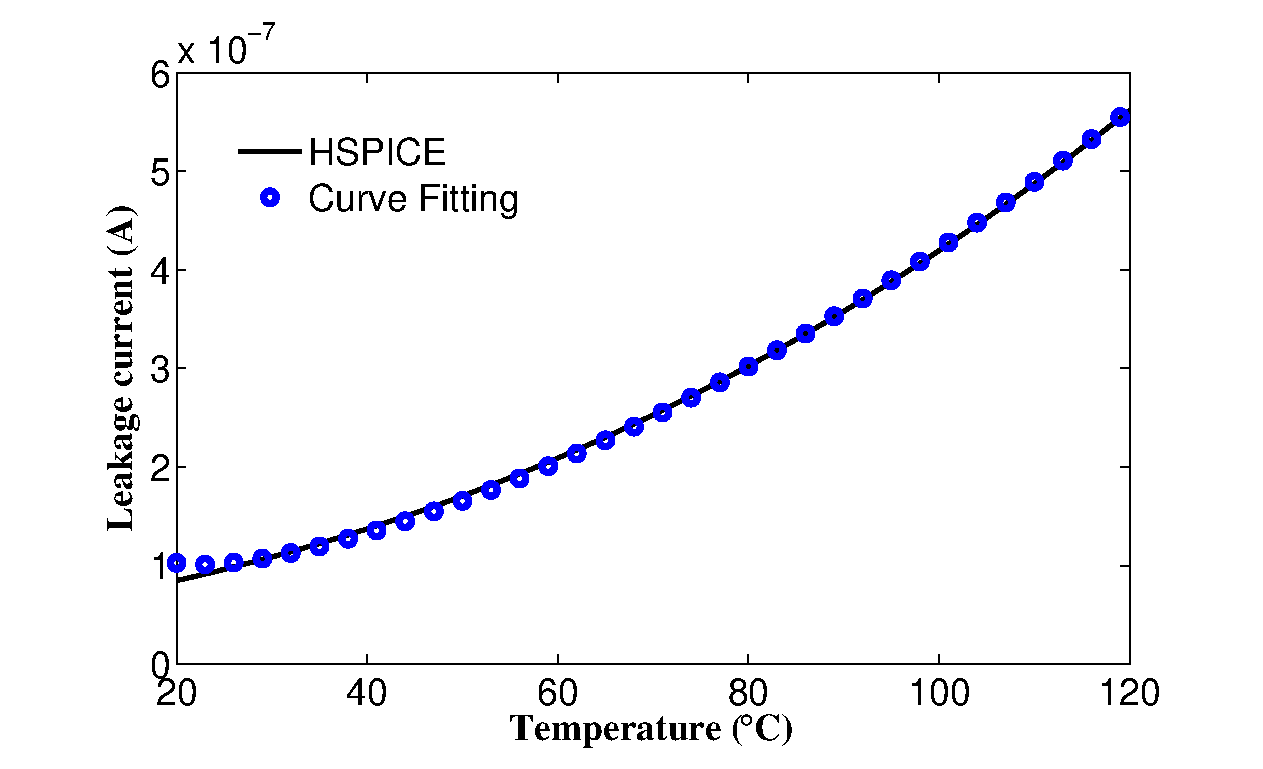
\includegraphics[width=1\columnwidth]{fig/leakage.eps}
%   \caption{Comparison of leakage of a TSMC \SI{65}{nm} process MOSFET from HSPICE
%     simulation with its curve fitting result using \eqref{eq:sub_current}. An example of
%     temperature region division is also shown in the figure, which will be discussed later.}
%   \label{fig:leakage}
% \end{figure}

\begin{figure}
  \centering
  \subfigure[Side view of the chip package structure]{
  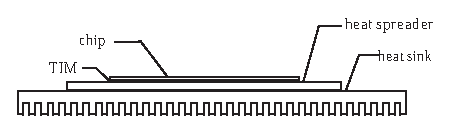
\includegraphics[width=0.7\columnwidth]{fig/chip_model.eps}
  \label{fig:chip_struct}}
  \subfigure[Floorplan example of a 16-core dark silicon chip.]{
  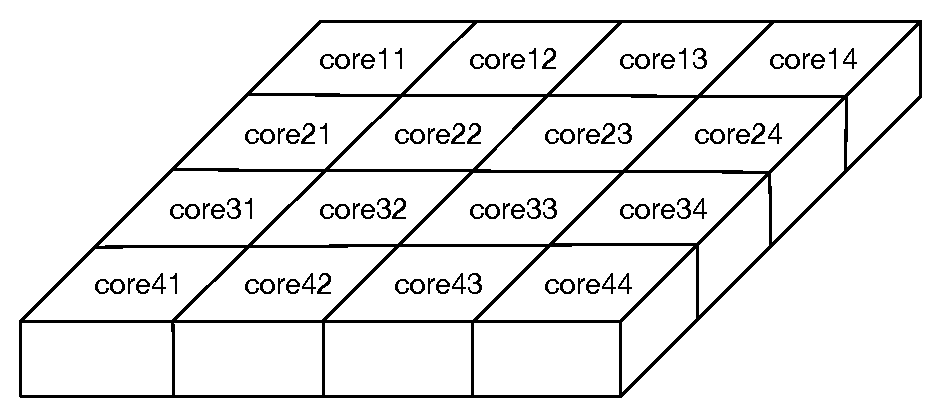
\includegraphics[width=0.6\columnwidth]{fig/16-core.eps}
  \label{fig:core_flp}}
\caption{Typical structure of a
    packaged multi-core dark silicon system.}
\end{figure}

\subsection{Thermal model}\label{sec:therm_model}
In this work, the multi-core dark silicon system is packaged in a common structure in Fig.~\ref{fig:chip_struct}. 
Heat (power) generated from the chip is conducted through thermal interface material (TIM), heat spreader, heat sink, and finally dissipated to the air through convection. The secondary heat path is ignored hear, since much fewer heat is dissipated through that path.

To estimate the power consumption of a IC chip, we first divide the chip and its package into multiple blocks called thermal nodes, with partition granularity determined by the accuracy requirements. For the dark silicon multi-core system (a 16-core chip's floorplan example is shown in Fig.~\ref{fig:core_flp}), we treat each core as a thermal node with a current source, because each core has very small area and highly correlated internal power distribution. The other thermal nodes from the package are divided according to the chip thermal nodes. Then, the thermal resistance and capacitance among these thermal nodes are determined, which model the thermal transport and power response behaviors. Please note that multi-core system floorplan different from the one shown in Fig.~\ref{fig:core_flp} are fully compatible with this work, and each core's internal structure can also be modeled if necessary. With above mentioned information, the thermal model for a chip with $n$ total thermal nodes can be generated:
\begin{equation}\label{eq:therm_model}
\begin{split}
GT(t) + C\frac{dT(t)}{dt} &= BP(t)\\
T_{c}(t) &= B^{T}T(t)
\end{split}
\end{equation}
where $T(t) \in \mathbb{R}^m$ is the temperature rise vector , representing temperature rise (from the ambient temperature) at $m$ places of the chip and package; $G \in \mathbb{R}^{m\times m}$ and  $C \in \mathbb{R}^{m \times m}$ contain equivalent thermal resistance and capacitance information respectively; $B \in \mathbb{R}^{m \times n}$ stores the information of how powers are injected into the thermal nodes; $P(T, t) \in \mathbb{R}^{n}$ is the power vector, which contains power consumptions of $l$ components on chip, including both dynamic power vector $P_d$ and static power vector $P_s$, i.e., $P(T, t)=P_s(T, t)+P_d(t)$. $T_{c}(t) \in \mathbb{R}^n$ is the output temperature vector, containing only temperatures of cores only. For detailed structure of $G$, $C$, and $B$ matrices, please refer to the thermal modeling works such as~\cite{Huang:TVLSI'06,Huang:TC'08,WangTan:TODAES'13,Hanumaiah:TCAD'11}.